\documentclass[MathsNotesBase.tex]{subfiles}




\date{\vspace{-6ex}}


\begin{document}

\chapter{Algebra}
\searchableSubsection{\chapterTitle{Algebra}}{abstract algebra, complex numbers}{\bigskip\bigskip}

	\searchableSubsection{\sectionTitle{Abstract Algebra}}{abstract algebra}{\bigskip}
	
	\bigskip\bigskip
	\searchableSubsection{Groups}{abstract algebra}{\bigskip
		
		\boxeddefinition{
		A binary operation is a function,
		\[ f:G \times G \longmapsto G \]
		which - by the definition of a function - maps a unique tuple from $G \times G$ to a unique value in the codomain $G$.
		}
		\bigskip
		
		\boxeddefinition{
		Let $G$ be a set and $*$ a binary operation on $G$ and denote this ($G,*$). Then ($G,*$) is a \textbf{group} if:
		\paragraph*{closure} $\forall x,y \in G, x * y \in G$;
		\paragraph*{associativity} $\forall x,y,z \in G, (x * y) * z = x * (y * z)$;
		\paragraph*{identity} $\exists e \in G \suchthat \forall x \in G, e*x = x*e = x$;
		\paragraph*{inverse} $\forall x \in G, \exists x^{-1} \in G \suchthat x * x^{-1} = x^{-1} * x = e$.\\\\
		These are known as the \textbf{group axioms}.
		}
		
		
		
		\bigskip\smallskip
		\boxeddefinition{
		The group is an \textbf{Abelian group} if it has the additional property:	
		\paragraph*{commutativity} $\forall x,y \in G, x * y = y * x \in G$.
		}
		
		\bigskip\smallskip 
		\notation{from here on we will use juxtaposition notation for the group operation (so $xy = x * y$) and (usually) $1$ for the identity element instead of $e$. This is known as \textit{multiplicative notation}.}
		
		\bigskip\bigskip
		\subsubsection{Corollaries of the group axioms}
		The group operation is defined to map a unique tuple in $G \times G$ to a unique value in $G$ so that if we have $x,y \in G$ then $f((x, y)) = f(x,y) = xy \in G$ and for $a,b,c \in G$,
		\[ a = b \iff (c, a) = (c, b) \implies f((c, a)) = f((c, b)) \iff ca = cb \]
		\[ \therefore a = b \implies ca = cb \]
		
		Then, using all the group axioms - associativity, inverse and identity,
		\[ ca = cb \implies \inv{c}(ca) = \inv{c}(cb) \iff (\inv{c}c)a = (\inv{c}c)b \iff 1a = 1b \iff a = b \]
		
		Therefore we have the principle of cancellation,
		\[ ca = cb \implies a = b \]
		\textit{Note} that, since we have used the axioms of inverse and identity and the definitions of these require these elements to exhibit these properties from both the left and the right, the principle of cancellation can also be shown from both the left and the right. So, also,
		\[ ac = bc \implies a = b \]
		
		\bigskip\bigskip
		There are (at least) two approaches to finding the other consequences of the group axioms.
		\paragraph*{First approach.} We begin by noticing that the law of cancellation implies that,
		\subparagraph*{unique identity and inverses}$\forall a,x,b \in G, ax = b$ has a unique solution because,
		\[ ax = ax' \iff x = x' \]
		That unique solution is $a^{-1}b$. If $b=a$ we have $ax=a$ and $x$, by identity axiom, is an identity element. Since, the solution to this equation - $x$ - is unique, it follows that there is a unique value that is the identity element. Then, if we let $b$ be this unique identity element we have $ax=1$ and the unique solution, $x$, is the inverse of a, i.e. $\inv{a}$. Therefore, the inverses of group elements are also unique.
		
		\paragraph*{Second approach.} This approach begins by showing the uniqueness of the identity element solely using the defintion of the identity. Here, for clarity, we revert to using $e$ to denote the identity element.
		\subparagraph*{unique identity} Assume there are two identity elements, $e, e'$. Then, by the definition of the identity $ee' = e'e = e = e'$ so that there is a single value that has the property of the identity element.\\\\
		Then, using the definition of the inverse we have,
		\subparagraph{unique inverses} Assume there are two distinct inverses of an element $a$: $\inv{a}$ and $a'$. Then, 
		\begin{align*}
		&& a\inv{a} = 1 &= aa' &\sidecomment{defn. of inverse, uniqueness of identity}\\
		& \iff & \inv{a} &= a' &\sidecomment{law of cancellation}
		\end{align*}
		\bigskip\bigskip

		\paragraph*{Some Examples of Groups}
		\begin{itemize}
		\item{ ($\R{} \setminus \{0\}, \times)$ } is a group whereas ($\R{}, \times)$ is not a group because $0$ has no multiplicative inverse.
		\item{ ($\R{}, +)$ } is a group.
		\item{ The set of $n \times n$ invertible matrices is called the General Linear group and denoted $GL_n$  }
		\item{Let $G$ denote the set of matrices
			\[ G = \left\{
				\begin{pmatrix}
					a & b \\
					0 & 1
				\end{pmatrix}
			\; \middle\vert \; a,b \in \Z{}_7, \; a \neq 0 \right\}. \]
			Then $G$ is a group with respect to matrix multiplication (where all additions and multiplications are carried out in $\Z{}_7$). This is because closure can be shown by,
			\[
				\begin{pmatrix}
				a & b \\
				0 & 1
				\end{pmatrix}
				\begin{pmatrix}
				a' & b' \\
				0 & 1
				\end{pmatrix}
				=
				\begin{pmatrix}
				aa' & ab' + b \\
				0 & 1
				\end{pmatrix} \in G
			\]
			where the result is in $G$ because ${ aa' \neq 0 }$. Next we need to show that we have inverses. So we need to show existence in $G$ of matrices such that,
			\[
				\begin{pmatrix}
				a & b \\
				0 & 1
				\end{pmatrix}
				\begin{pmatrix}
				a' & b' \\
				0 & 1
				\end{pmatrix}
				=
				\begin{pmatrix}
				1 & 0 \\
				0 & 1
				\end{pmatrix} 
				\iff
				\begin{pmatrix}
				aa' & ab' + b \\
				0 & 1
				\end{pmatrix}
				=
				\begin{pmatrix}
				1 & 0 \\
				0 & 1
				\end{pmatrix}
			\]
			which implies that ${ aa' = 1 }$ and ${ ab' + b = 0 }$. Because we are in $\Z{}_7$ every non-zero element has a multiplicative inverse so we have,
			\[ a' = \inv{a} \eqand b' = -\inv{a}b \]
			so that,
			\[
				\inv{\begin{pmatrix}
				a & b \\
				0 & 1
				\end{pmatrix}}
				=
				\begin{pmatrix}
				\inv{a} & -\inv{a}b \\
				0 & 1
				\end{pmatrix}.
			\]
		}
		\end{itemize}
		
		\bigskip
		\subsubsection{Permutations and Symmetric Groups}\bigskip
		\boxeddefinition{
			A \textbf{permutation} is a bijection from a set to itself. Since permutations are bijective, they are invertible and since they are functions, function composition defines an associative law of composition over them. As a result, they form a group. 
		}
		\boxeddefinition{
			The \textbf{symmetric group} defined over a set is the group whose elements are the permutations of the objects of the set and whose law of composition is the composition of functions. The name probably comes from the study of symmetries of geometric objects that were eventually realised to be equivalent to permutations of the vertices.
		}
		\notation{The symmetric group over the integers from 1 to n is denoted $S_n$.}\\
		\subparagraph{$\bm{S_2}$}
		The symmetric group $S_2$ consists of the two elements $i$ and $\tau$ which are, respectively, the identity map and the transposition which interchanges 1 and 2. The group composition law is described by the fact that the identity map is the identity of the composition and by the relation $\tau\tau = \tau^2 = i$. Which results in the multiplication table:	
		\[
		\begin{aligned}
			i &\cdot i &&= i \\
			i &\cdot \tau &&= \tau \\		
			\tau &\cdot i &&= \tau \\
			\tau &\cdot \tau &&= i \\
		\end{aligned}
		\]
		Note that the law of composition is commutative.
		\subparagraph{$\bm{S_3}$}\label{S_3}
		The symmetric group $S_3$ contains $3!$ elements. It is the smallest group whose law of composition is not commutative. It can be described using any two permutations of $\{1, 2, 3\}$. For example, if we take,
		\begin{align*}
			x =
			\begin{bmatrix}
			0 & 1 & 0 \\
			0 & 0 & 1 \\
			1 & 0 & 0 \\
			\end{bmatrix},\;
			y =
			\begin{bmatrix}
			0 & 1 & 0 \\
			1 & 0 & 0 \\
			0 & 0 & 1 \\
			\end{bmatrix}
		\end{align*}
		Then the permutations are,
		\[ \{1, x, x^2, y, xy, x^2y\} = \setc{x^iy^j}{0 \leq i \leq 2,\; 0 \leq j \leq 1} \]
		These are the elements of the group. The composition law over these elements is the function composition of these permutation functions and its multiplication table is characterized by the rules:
		\begin{align*}
			x^3 = 1,\; y^2 = 1,\; yx = x^2y
		\end{align*}
		These are derived directly from the permutations themselves. Note that this composition law is not associative as $yx \neq xy$. \\
		Any product of the elements $x,y$ and of their inverses can be brought into the form $x^iy^j$ with $i,j$ taking the ranges given above by repeated application of the above rules. To do so, we move all occurrences of $y$  to the right side using the last relation and bring the exponents into the indicated ranges using the first two relations:
		\begin{align*} 
			\inv{x}y^3x^2y &= x^2yx^2y = x^2(yx)xy = x^2(x^2y)xy = x^4(yx)y\\
						&= x^4(x^2y)y = x^6y^2 = (x^3)^2y^2 = 1 \cdot 1 = 1
		\end{align*}
		Rules like these that determine a complete multiplication table are called \textit{defining relations} for the group.	
	}
	
	
	\pagebreak
	\searchableSubsection{Subgroups}{abstract algebra}{\bigskip
		\boxeddefinition{
			A subset $H$ of a group $G$ is called a \textbf{subgroup} if it has the following properties:
			\begin{itemize}
				\item{\textbf{Closure:}} If $a \in H$ and $b \in H$ then $ab \in H$.
				\item{\textbf{Identity:}} $1 \in H$.
				\item{\textbf{Inverses:}} If $a \in H$ then $\inv{a} \in H$.
			\end{itemize}
			\note{These conditions show that the subset $H$ is a group with respect to the \textit{induced law of composition} created by applying the law of composition of $G$ on the members of $H$. Note that the associative property is not mentioned because the associativity of the composition of members of $G$ automatically carries over to $H$.}
		}
		
		
		\notation{If $H$ and $G$ are groups then we may write ${ H \leq G }$ to indicate that $H$ is a subgroup of $G$.}\\\\
		
		\note{Note that an alternative, more compact, formulation of the definition of a subgroup is as follows.\\\\
			\textbf{Let $\bm{G}$ be a group and ${\bm{ \emptyset \neq H \subseteq G }}$. Then $\bm{H}$ is a subgroup if}
			\[ \bm{ x,y \in H \implies \inv{x}y \in H }. \]
			This is because,
			\[ [(x,y \in H \implies xy \in H) \wedge (x \in H \implies \inv{x} \in H)] \iff (x,y \in H \implies \inv{x}y \in H). \]
			The implication,
			\[ [(x,y \in H \implies xy \in H) \wedge (x \in H \implies \inv{x} \in H)] \implies (x,y \in H \implies \inv{x}y \in H) \]
			is obvious. In the other direction,
			\[ (x,y \in H \implies \inv{x}y \in H) \implies [(x,y \in H \implies xy \in H) \wedge (x \in H \implies \inv{x} \in H)] \]
			is because, if we set ${ x = y }$,
			\[ \inv{x}x = e \in H \implies \inv{x}e = \inv{x} \in H \]
			and then, for ${ x \neq y }$,
			\[ \inv{x},y \in H \implies xy \in H. \]
		}
		

		Every group, at a minimum, has two trivial subgroups: the maximal subgroup - the group itself; and the minimal subgroup - the set containing just the identity. A subgroup that is neither of these is known as a \mbox{\textit{proper subgroup}}.\\\\

		
		Important examples are the subgroups of the additive group of integers $\Z{+}$. Denote the subset of $\Z{+}$ consisting of all multiples of a given integer $b$ by $b\Z{}$ such that,
		\[ b\Z{} = \setc{n \in \Z{}}{n = bk,\; k \in \Z{}} \]
		\labeledProposition{For any integer $b$, the subset $b\Z{}$ is a subgroup of $\Z{+}$ and every subgroup of $\Z{+}$ is of the form $b\Z{}$ for some integer $b$.}{bZ_subgroup}
		\begin{proof}
			$b\Z{}$ is a subgroup of $\Z{+}$ because,
			\begin{itemize}
				\item{$b(0) = 0 \in b\Z{}$;}
				\item{If $a_1,a_2 \in b\Z{}$ then $a_1 = bk_1, a_2 = bk_2$ for $k_1, k_2 \in \Z{}$ and so $a_1 + a_2 = bk_1 + bk_2 = b(k_1 + k_2) \in b\Z{}$}
				\item{For any $a = bk \in b\Z{}$, $-a = b(-k) \in b\Z{}$}
			\end{itemize}
			Now we need to prove that any subgroup of $\Z{+}$ is $b\Z{}$ for some $b$. Let $H$ be an arbitrary subgroup of $\Z{+}$. Then by subgroup properties,
			\begin{itemize}
				\item{$0 \in H$;}
				\item{If $a_1,a_2 \in H$ then $a_1 + a_2 \in H$}
				\item{For any $a \in H$, $-a \in H$}
			\end{itemize}
			We proceed to show that there is always some integer $b$ such that $H = b\Z{}$.\\
			Firstly, if $H$ is the minimal subgroup \{0\} then $H$ trivially conforms to $b\Z{}$ with $b = 0$.\\
			Otherwise, $\exists a \in H \suchthat a \neq 0$ then also $\exists -a \in H \suchthat -a \neq 0$. One of these must be a positive non-zero integer so there is at least one such member of $H$. We take $b$ to be the smallest positive non-zero integer in $H$. Then,
			\paragraph{$\bm{b\Z{} \in H}$}
			\begin{itemize}
				\item{$b \in H$ (by selection) so by subgroup properties $b + b \in H$ and $(b + b) + b \in H$ and $b + \cdots + b \in H$}
				\item{By subgroup properties $b \in H \implies -b \in H$}
			\end{itemize}
			So, $\setc{bk \in \Z{}}{k \in \Z{}}$ is in $H$.
			\paragraph{$\bm{H \in b\Z{}}$}
			Take any $n \in H$. Using division with remainder and dividing by $b$ we get,
			\[ n = bq + r \;\; q \in \Z{},\, 0 \leq r < b \]
			But, since $b\Z{} \in H$ this means that $bq \in H$ and so $-bq \in H$. Therefore $n - bq = r \in H$. But $0 \leq r < b$ and, by assumption, $b$ is the smallest positive \textit{non-zero} integer in $H$ and so, $r = 0$. So, every $n \in H$ divides by $b$.
		\end{proof}
	
		\subsubsection{Greatest Common Divisor}
		If we extend this to groups which are generated by two integers $a,b$, then we have a subgroup of $\Z{+}$,
		\[ a\Z{} + b\Z{} = \setc{n \in \Z{}}{n = ar + bs \;\; r, s \in \Z{}} \]
		This is known as the subgroup \textit{generated} by $a,b$ because it is the smallest subgroup which contains $a$ and $b$. \autoref{prop:bZ_subgroup} tells us that it has the form $d\Z{}$ for some integer $d$.
		\begin{corollary}
			\label{coro:greatest_common_divisor}
			If $d$ is the positive integer which generates the subgroup $a\Z{} + b\Z{}$ then $d$ is the greatest common divisor of $a$ and $b$ and so,
			\begin{itemize}
				\item{$d$ can be written in the form $d = ar + bs$ for some integers $r$ and $s$.}
				\item{$d$ divides $a$ and $b$.}
				\item{If an integer $e$ divides $a$ and $b$, it also divides $d$.}
			\end{itemize}
		\end{corollary} 
		\begin{proof}
			The first property follows directly from the definition of the subgroup. The second property is a result of the fact that $a,b$ are in the subgroup $a\Z{} + b\Z{}$ so that $d\Z{} = a$ and $d\Z{} = b$. The third property is evident because $d = ar + bs = ek_1r + ek_2s = e(k_1r + k_2s)$.
		\end{proof}
	
	
		\labeledProposition{Suppose ${ G = \{g_1, g_2, \dots , g_n\} }$ is a finite group of order $ n $ and that ${ x \in G }$. Then ${ \{xg_1, xg_2, \dots , xg_n\} = G }$.}{coset_of_group_with_element_in_group_is_identical_to_group}
		\begin{proof}
			Let ${ X = \{xg_1, xg_2, \dots , xg_n\} }$. By closure in G, every element of $X$ must be in $G$ and by the inverses property in $G$ every element of $X$ is distinct. So, there are $n$ distinct elements of $X$, each of which are members of $G$. Since the order of $G$ is $n$ we can conclude that ${ X = G }$.
		\end{proof}
	
		\labeledProposition{Suppose that $G$ is a finite group and that $H$ is a non-empty subset of $G$ such that ${ x,y \in H \implies xy \in H }$. Then $H$ is a subgroup.
		}{closed_subset_of_finite_group_is_subgroup}
		\begin{proof}
			$H$ is non-empty so it contains at least one element, say ${ x }$. $H$ is closed under the group operation so it must also contain ${ x^2, x^3, \dots }$. But $G$ is finite so the order of $x$ in G must be finite also and so ${ \exists n \in \N{} \suchthat x^n = e }$. But also ${ x^n = e \iff x^{n-1} = \inv{x} }$. Therefore, for every element in $H$, the inverse of the element is also in $H$.
		\end{proof}
	
		\labeledProposition{Suppose that $p$ is a prime number and we have integers ${ 1 \leq x,g,h < p }$ such that ${ xg \equiv xh \modulo{p} }$. Then ${ g = h }$ and ${ x \in \Z{*}_p }$ has an inverse.}{modulo_of_primes_have_inverses}
		\begin{proof}
			If ${ xg \equiv xh \modulo{p} }$ then the difference between $xg$ and $xh$ is a multiple of $p$. But Euclid's Lemma (\url{https://en.wikipedia.org/wiki/Euclid's_lemma}) tells us that ${ p \divides (xg - xh) = x(g - h) \implies (p \divides x) \wedge (p \divides (g-h)) }$. But since we have ${ x,(g-h) < p }$ it is impossible for $p$ to divide either of them unless they are 0. Only ${ g-h }$ can be 0. Therefore,
			\[ g - h = 0 \iff g = h. \]
			So, if we define a function ${ f: \Z{*}_p \longmapsto \Z{*}_p }$ such that ${ f(a) = xa }$ for some fixed ${ x \in \Z{*}_p }$ then $f$ is injective because
			\[ f(a) = f(b) \iff xa \equiv xb \modulo{p} \iff a \equiv b \modulo{p}. \]
			This means that $f$ maps the ${ p-1 }$ different values of ${ \Z{*}_p }$ to ${ p-1 }$ different values in ${ \Z{*}_p }$. Therefore $f$ is a bijection and there exists an inverse function ${ \inv{f} }$ such that ${ \inv{f}(xa) = a }$.
		\end{proof}
	
		\medskip
		\subsubsection{Examples of Subgroups}
		\begin{exe}
			\ex{${ (\Z{*}_p, \otimes) }$ for prime $p$ is a subgroup of the integers. This can be seen as closure of modular multiplication is clear and the existence of inverses has been shown in \autoref{prop:modulo_of_primes_have_inverses}.\\
			This is not the case however, for non-prime p. For example ${ (\Z{*}_6, \otimes) }$ is not a subgroup as it does not have inverses. We can see this by looking at the values generated by selecting a non-identity element and multiplying it by all the elements in ${ \Z{*}_6 }$:
			\[ 2 \otimes 1 = \bm{2},\; 2 \otimes 2 = \bm{4},\; 2 \otimes 3 = \bm{0},\; 2 \otimes 4 = \bm{2},\; 2 \otimes 5 = \bm{4}. \]
			As can be seen, it doesn't generate all the values of ${ \Z{*}_6 }$ but repeats a subset of them. Compare with the same for ${ \Z{*}_7 }$:
			\[ 2 \otimes 1 = \bm{2},\; 2 \otimes 2 = \bm{4},\; 2 \otimes 3 = \bm{6},\; 2 \otimes 4 = \bm{1},\; 2 \otimes 5 = \bm{3},\; 2 \otimes 6 = \bm{5}. \]
			In the case of prime $p$ all the values are generated so that multplication by other elements is a bijective function with a corresponding inverse.
			}
			\ex{\medskip Let R be a non-square rectangle in $\R{2}$ with corners having coordinates ${ (-1,-1), (-1,2), (1,2), (1,-1) }$. Then there are four symmetries ${ i,a,b,c }$ of R, as follows:\medskip
				\begin{itemize}
					\item{$i$ is the identity}
					\item{$a$ is reflection in the $x$-axis}
					\item{$b$ is reflection in the $y$-axis}
					\item{$c$ is a rotation of $\pi$ radians around the origin.}
				\end{itemize}
				\begin{figure}[h!]
					\centering
					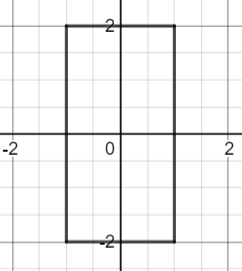
\includegraphics{resources/img/subgroup_example_rectangle_symmetries.png}
					\par
				\end{figure}
				These symmetry operations form a group whose group table is as follows.
				\begin{table}[h!]%
					\centering%
					\begin{tabular}{|c||c|c|c|c|}
						\hline
							&  $i$  & $a$   & $b$ & $c$ \\
						\hline
						\hline
						$i$ &  $i$  & $a$   & $b$ & $c$ \\
						\hline
						$a$ & $a$   & $i$ 	& $c$ & $b$ \\
						\hline
						$b$ & $b$ 	& $c$   & $i$ & $a$ \\
						\hline
						$c$ & $c$ 	& $b$ 	& $a$ & $i$ \\
						\hline
					\end{tabular}
				\end{table}
			}
		\end{exe}
	
		\bigskip
		\subsubsection{Cyclic Subgroups}
		\boxeddefinition{
			If we take a single member of a group (along with its inverse and the identity), the subgroup generated by that element takes the form (using multiplicative notation),
			\[ H = \{ x^{-(n-1)},\, \cdots , x^{-2}, x^{-1}, 1, x, x^2,\, \cdots , x^{n-1} \} \]
			where, either, $x^n = 1$ so that there are $n$ distinct values in the group, or else $n$ is infinite and the values never repeat.
			This is known as a \textbf{cyclic group} and also as the \textbf{subgroup generated by $\bm{x}$} and is denoted by $\langle x \rangle$.
		}
		\note{The cyclic subgroup, $\langle x \rangle$, generated by $x$ is the smallest subgroup of $G$ containing $x$ in the sense that, if ${ H \leq G }$ and ${ x \in H }$ then ${ \langle x \rangle \subseteq H }$.}
		
		
		\labeledProposition{The set $S$ of integers $n$ such that $x^n = 1$ is a subgroup of $\Z{+}$}{cyclic_powers_add_subgroup_integers}
		\begin{proof}
			If $x^m = 1$ and $x^n = 1$, then $x^{m+n} = x^mx^n = 1$ also so we have closure of addition. Since $x^0 = 1$, 0 is in the subgroup so we have an identity. Finally, for some $n$ in the subgroup, $x^n = 1 \iff x^{-n} = x^nx^{-n} = x^0 = 1$ so $n$ being in the subgroup implies that $-n$ is also in the subgroup and we have inverses.
		\end{proof}
		\begin{corollary}
			It follows from $S$ being a subgroup of $\Z{+}$ and from \autoref{prop:bZ_subgroup} that $S$ has the form $m\Z{}$ where $m$ is the smallest positive integer such that $x^m = 1$. Therefore, in $H$, the $m$ elements $1, x, x^2, \cdots , x^{m-1}$ are all different and any element in $H$ will simplify to one of them: for $n \in S$, $n = mq + r$ such that $x^n = (x^m)^qx^r = 1^qx^r = x^r$.
		\end{corollary}
		
		\boxeddefinition{The \textbf{order} of a group $G$ is the number of distinct elements it contains. It is typically denoted $\vert G \vert$.\\
			An element of a group is said to have \textbf{order} $m$ (possibly infinity) if the cyclic subgroup it generates has order $m$. This means that $m$ is the smallest positive integer with the property $x^m = 1$ or, if the order is infinite, that, $x^m \neq 1$ for all $m \neq 0$.
		}
	
		\labeledTheorem{A group of finite order cannot have any element of infinite order.}{finite_group_no_infinite_order_element}
		\begin{proof}
			If $G$ is a group and ${ x \in G }$ has infinite order then,
			\begin{align*}
			&& x^m &= x^n \\
			&\iff & x^{m-n} &= 1= x^{n-m} &\sidecomment{} \\
			&\iff & x^{\abs{m-n}} &= 1 &\sidecomment{} \\
			&\therefore & \abs{m-n} &= 0. &\sidecomment{because order of x is infinite} \\
			\end{align*}
			So, there are no two distinct powers of $x$ that produce the same object so that ${ \langle x \rangle \leq G }$, the cyclic group generated by $x$, is infinite. Since ${ \langle x \rangle \subseteq G }$ this requires that $G$ also be infinite.
		\end{proof}
	
		\bigskip
		\labeledTheorem{If a group element $x$ has finite order $m$ then:
			\begin{enumerate}
				\item{Let ${ n \in \Z{}. }$ If ${ n = km + r }$ where ${ k,r \in \Z{} }$ and ${ 0 \leq r \leq m - 1 }$, then ${ x^n = x^r. }$}
				\item{For ${ n \in \N{},\; x^n = 1 \iff m | n. }$}
				\item{${ 1,x,x^2,\dots,x^{m-1} }$ is a complete, repetition-free, list of elements of ${ \langle a \rangle. }$}
				\item{The subgroup ${ \langle a \rangle }$ generated by $x$ has cardinality $m$.}
			\end{enumerate}
		}{finite_order_group_element_properties}
	
		\subsubsection{Examples of Cyclic Subgroups}
		\bigskip
		\begin{exe}
			\ex{\textbf{Cyclic group with order 3}
				\[ G = \{1, x, x^2\} \]
				where $x^3 = 1$ is a cyclic group of order 3 generated by the element $x$. Note that, since this is a group, it must also contain the inverses, $x^{-1}, x^{-2}$ but ${ x^3 = 1 }$ so ${ x^{-1} = x^2 }$ and ${ x^{-2} = x }$.\\
			}
			\ex{\textbf{Symmetries of an equilateral triangle}\\\\
				Consider an equilateral triangle with vertices labeled ${ A,B,C }$:
				\begin{align*}
		  		& A &  \\
				B & \hspace{7pt} C. & \\
				\end{align*}
				Every permutation of the vertices is a transformation that produces an object that occupies the same space as the original, i.e. a \textit{symmetry}. If we take one of them, say, the clockwise rotation one place that results in,
				\begin{align*}
				& B &  \\
				C & \hspace{7pt} A & \\
				\end{align*}
				and we name this $r$, then clearly -- since there are 3 vertices -- performing this same rotation 3 times leaves us back where we started. So, using function composition as the law of composition and multiplicative notation, $r^3 = i$ where $i$ is the identity transformation. Also the inverse of $r$ is $r^2$. So, we have a group consisting of ${ \{i, r, r^2\} }$ and function composition. Notice the resemblance of this group to the previous group ${ \{1, x, x^2\} }$; this group is \textit{isomorphic} to the cyclic group of order 3.\\
			}
			\ex{\textbf{Group ${\bm{ (\Z{*}_5, \otimes) }}$}\\\\
				Consider the element 2 modulo 5. Using multiplicative notation we have,
				\[ 2^2 = 4, 2^3 = 8 = 3, 2^4 = 16 = 1, 2^5 = 32 = 2. \]
				So ${ 2^1 = 2^5 \iff 1 = 2^4 }$ meaning that the element 2 has order 4 in the group and we see, as expected that the group it generates, ${ \langle 2 \rangle }$ has 4 members. In this case, the members are all the members of the group -- that's to say, \textit{the element 2 generates the whole group}. If we consider the element 4 we have,
				\[ 4^2 = 16 = 1, 4^3 = 64 = 4. \]
				So this element oscillates between 1 and 4 and so, the cyclic subgroup that it generates ${ \langle 4 \rangle }$ has order 2.\\
				Since the group ${ (\Z{*}_5, \otimes) = \langle 2 \rangle }$ it can also be described as a cyclic group. This will be the case for any such group modulo a prime number -- i.e. ${ (\Z{*}_p, \otimes) }$ where $p$ is prime.\\
			}
			\ex{\textbf{Cyclic group with infinite order}
				\[
				\begin{bmatrix}
				1 & 1	\\
				0 & 1 	\\
				\end{bmatrix} 
				\]
				under matrix multiplication (which is commutative in this case), generates a cyclic group of infinite order because
				\[
				\begin{bmatrix}
				1 & 1	\\
				0 & 1 	\\
				\end{bmatrix}^n =
				\begin{bmatrix}
				1 & n	\\
				0 & 1 	\\
				\end{bmatrix}.
				\]
				\smallskip
			}
			\ex{\textbf{The Klein Four Group, $V$} is the simplest group that is not cyclic (it cannot be generated by a single element). It appears in many forms but, as an example, it can be realized as the group consisting of the four matrices,
				\[
				\begin{bmatrix}
				\pm 1 & 0 		\\
				0 & \pm 1 	\\
				\end{bmatrix} 
				\]
				Any two non-identity elements generate $V$.
			}
		\end{exe}
	}

	
	\bigskip\bigskip
	\searchableSubsection{Isomorphisms}{abstract algebra}{\bigskip
		\boxeddefinition{An \textbf{isomorphism} is a bijection between two groups that preserves the structure of the groups by being compatible with the law of composition of both groups. More formally, two groups are \textbf{isomorphic} if there exists a bijection $\phi : G \longmapsto G'$ such that,
			\[ \phi(ab) = \phi(a)\phi(b) \text{ for all } a,b \in G \]
			where $ab$ represents composition according to the law of composition of $G$ and $\phi(a)\phi(b)$ represents composition according to the law of composition of $G'$.
		}
	
		\note{An \textbf{isomorphism} is a \textbf{bijection} between two \textbf{groups}. That's to say, it is already assumed in the definition of an isomorphism that the codomain $G'$ is a group.}
	
		\labeledProposition{As a consequence of this sole property that, across the bijection, the respective laws of composition are preserved, all other properties of the groups are also preserved.}{isomorphism_preserves_structure}
		\begin{proof}
			Let $e$ be the identity in $G$ and $e' = \phi(e) \in G'$, and $1'$ be the identity element in $G'$ then,
			\begin{itemize}
				\item{
					Since $G'$ is a group, it has the inverses property that every element has an inverse so,
					\begin{align*}
						 &&e' &= \phi(e) = \phi(ee) = \phi(e)\phi(e) = e'e' &\sidecomment{using preservation of law of composition}\\
						 &\iff &\inv{(e')}e' &= (\inv{(e')}e')e' &\sidecomment{using the inverses property of $G'$}\\
						 &\iff &1' &= e'
					\end{align*}
					which implies that $e'$ is the identity in $G'$ so that $\phi$ maps the identity in $G$ to the identity in $G'$.}
				\item{We can use the fact just shown that $\phi(e) = e' = 1'$ to show,
					\begin{align*}
						&&1' = e' = \phi(e) &= \phi(a\inv{a}) = \phi(a)\phi(\inv{a}) &\sidecomment{using preservation of law of composition}\\
						&\iff &\inv{\phi(a)}1' &= \inv{\phi(a)}\phi(a)\phi(\inv{a}) &\sidecomment{using the inverses property of $G'$}\\
						&\iff &\inv{\phi(a)} &= \phi(\inv{a})
					\end{align*}
					which shows that $\phi$ maps $\inv{a} \in G$ to $\inv{\phi(a)} \in G'$.}
			\end{itemize}
		\end{proof}
		
		 For example, if $e \in G$ is the identity of $G$ mapped to an element $ e' = \phi(e) \in G' $, then for any $a \in G$ mapped to $a' = \phi(a) \in G'$,
		\[ a' = \phi(a) = \phi(ea) = \phi(e)\phi(a) = e'a' \]
		And $a' = e'a' = a'e'$ means that $e'$ is the identity in $G'$. Furthermore, the order of elements in $G$ and $G'$ will also be the same as,
		\[ a^n = e \iff e' = \phi(e) = \phi(a^n) = \phi(a)^n = (a')^n \]
		
		Since two isomorphic groups have the same properties, it is often convenient to identify them with each other when speaking informally. For example, the symmetric group $S_n$ of permutations of $\{1,\cdots,n\}$ is isomorphic to the group of permutation matrices, a subgroup of $GL_n(\R{})$ and we often blur the distinction between these two groups.\\
		
		\notation{Sometimes when two groups are isomorphic this is indicated using the notation,
			\[G \approx G'\]
		}
	
		\subsubsection{Examples}
		\begin{itemize}
			\item{
				Let $C = \{ \cdots, a^{-2}, a^{-1}, 1, a, a^2, \cdots \}$ be an infinite cyclic group. Then the map,
				\[ \phi : \Z{+} \longmapsto C \; \suchthat \; \phi(n) = a^n \]
				is an isomorphism where the preservation of the respective laws of composition can be seen as,
				\[ \phi(m + n) = a^{m + n} = a^ma^n = \phi(m)\phi(n) \]
				and also ${ n + (-n) = 0 }$ and,
				\[ \phi(-n) = a^{-n} = \inv{(a^n)}. \]
			}
			\item{Let $G$ be the set of real matrices of the form,
				\[
				\begin{bmatrix}
				1 & x 	\\
				0 & 1 	\\
				\end{bmatrix} 
				\]
				This is a subgroup of $GL_2(\R{})$ and so, its law of composition is the same as that of $GL_2(\R{})$, i.e. matrix multiplication.
				\[
				\begin{bmatrix}
				1 & x 	\\
				0 & 1 	\\
				\end{bmatrix}
				\begin{bmatrix}
				1 & y 	\\
				0 & 1 	\\
				\end{bmatrix} = 
				\begin{bmatrix}
				1 & x + y\\
				0 & 1 	\\
				\end{bmatrix}
				\]
				So, $G$ is isomorphic to $\R{+}$, the additive group of reals.
			}
		\end{itemize}
		
		\boxeddefinition{The groups isomorphic to a given group $G$ form what is called the \textbf{isomorphism class} of $G$. Groups are often classified into isomorphism classes, for example, there is one isomorphism class of groups of order 3 and there are two classes of groups of order 4 and five classes of 12.}
		
		\labeledProposition{There is only one isomorphism class for each order of cyclic group.}{one_class_per_cyclic_order}
		\begin{proof}
			Any two cyclic groups of the same order are isomorphic because, if
			\[ G = \{1, x, x^2, \cdots, x^{n-1}\}, \; G' = \{1, y, y^2, \cdots, y^{n-1}\} \]
			are two cyclic groups of order $n$ then the map $\phi(x^i) = y^i$ is an isomorphism.
		\end{proof}
		
		\subsubsection{Automorphisms}
		\boxeddefinition{The domain and codomain of an isomorphism can be the same set of objects so that $\phi : G \longmapsto G$. This is known as an \textbf{automorphism}.}
		\paragraph{Example}
		Let $G = \{1, x, x^2\}$ be a cyclic group of order 3 so that $x^3 = 1$. The transposition which interchanges $x$ and $x^2$ is an automorphism of $G$,
		\[\begin{array}{*6c}
			&1 &&\longmapsto &&1 \\
			&x &&\longmapsto &&x^2 \\
			&x^2 &&\longmapsto &&x \\
		\end{array}\]
		\begin{table}[h!]%
			\centering%
			\begin{tabular}{|c||c|c|c|}
				\hline
				      &  1    & $x$   & $x^2$ \\
				\hline
				\hline
				 1    &  1    & $x$   & $x^2$ \\
				\hline
				$x$   & $x$   & $x^2$ & 1     \\
				\hline
				$x^2$ & $x^2$ & 1     & $x$ \\
				\hline
			\end{tabular}
			$ \longmapsto $
			\begin{tabular}{|c||c|c|c|}
				\hline
				      &  1    & $x^2$ & $x$  \\
				\hline
				\hline
				1     &  1    & $x^2$  & $x$  \\
				\hline
				$x^2$ & $x^2$ & $x$   & 1    \\
				\hline
				$x$   & $x$   & 1     & $x^2$ \\
				\hline
			\end{tabular}
		\end{table}
		\\\\This is because the group is cyclic and $x$ and $x^2$ have the same order ($x^3 = 1$ and also $(x^2)^3 = x^6 = (x^3)^2 = 1^2 = 1$). So the law of composition is preserved.
		\paragraph{Conjugation}
		The most important example of automorphism is conjugation.\\\\
		\boxeddefinition{\textbf{Conjugation} by $b \in G$ is the map from $G$ to itself defined by,
			\[ \phi(a) = ba\inv{b} \]
			with the result that,
			\[ ba = \phi(a)b \]
			so that we can think of conjugation of $a$ by $b$ as the way that we need to change $a$ if we want to move the multiplication by $b$ to the other side.
		}
		This is an automorphism because it
		\begin{itemize}
			\item{is compatible with law of composition, 
				\[ \phi(xy) = bxy\inv{b} = bx\inv{b}by\inv{b} = \phi(x)\phi(y) \]
			}
			\item{has an inverse so it is bijective, 
				\[ (\inv{\phi} \circ \phi)(a) = \inv{\phi}(\phi(a)) = \inv{b}(ba\inv{b})b = (\inv{b}b)a(\inv{b}b) = a \]
				Note that this is different from the inverse element of $a$ corresponding under the mapping $\phi$,
				\[ \phi(a)\phi(\inv{a}) = ba\inv{b}b\inv{a}\inv{b} = ba(1)\inv{a}\inv{b} = b(1)\inv{b} = 1 \]
			}
		\end{itemize}
		Another thing to note is that - in an abelian group where the composition law is commutative - conjugation becomes the identity map,
		\[ ba = ab \iff ba\inv{b} = a \iff \phi(a) = a \]
	}

	
	\bigskip\bigskip
	\searchableSubsection{Homomorphisms}{abstract algebra}{\bigskip
		\boxeddefinition{A \textbf{homomorphism} is a mapping (not necessarily bijective) between two groups, $\phi : G \longmapsto G'$, such that,
			\[ \phi(ab) = \phi(a)\phi(b) \text{ for all } a,b \in G \]
			where $ab$ represents composition according to the law of composition of $G$ and $\phi(a)\phi(b)$ represents composition according to the law of composition of $G'$. 
		}
		So, the difference between a \textit{homomorphism} and a \textit{isomorphism} is that the latter is bijective whereas the former is not. As a result, a \textit{homomorphism} may be one-way only.\\
		
		\note{A \textbf{homomorphism} is a \textbf{mapping} between two \textbf{groups}. That's to say, it is already assumed in the definition of a homomorphism that the codomain $G'$ is a group.}
		
		\paragraph{Examples of homomorphisms}
		\begin{exe}
			\ex {	Let $C = \{ a^{n-1}, \cdots, a^{-2}, a^{-1}, 1, a, a^2, \cdots, a^{n-1} \}$ be a finite cyclic group. Then the map,
				\[ \phi : \Z{+} \longmapsto C \; \suchthat \; \phi(n) = a^n \]
				is a homomorphism. Note that if $C$ were an infinite cyclic group then this would be an isomorphism. }\label{ex_finite_cyclic_group}
			\ex {the sign of a permutation $ sign : S_n \longmapsto {\pm1} $}\label{ex_sign_permutation}
			\ex {the determinant function $ det : GL_n(\R{}) \longmapsto \R{\times} $}\label{ex_determinant}
			\ex {an arguably trivial example is called the \textit{inclusion} map $i : H \longmapsto G$ of a subgroup $H$ into a group $G$, defined by $i(x) = x$. It functions as the identity for elements in the subgroup $H$ but, since it is not surjective, there is no inverse mapping.}\label{ex_inclusion_map}
		\end{exe}
	
		
		
		\subsubsection{Image of a homomorphism}
		Since a homomorphism is not bijective it has an image different to the codomain group,
		\[ im \; \phi = \setc{x \in G'}{\exists a \in G \suchthat \phi(a) = x} \]
		The image of a homomorphism is a subgroup of the codomain group $G'$ because the homomorphism preserves the group structure as described in \autoref{prop:isomorphism_preserves_structure}.\\\\
		\notation{The image of the mapping $\phi$ with domain $G$ is sometimes denoted $\phi(G)$.}
		
		\subsubsection{Kernel of a homomorphism}
		\boxeddefinition{The \textbf{kernel} of a homomorphism is the set of elements in the domain that are mapped to the identity,
			\[ ker \; \phi = \setc{a \in G}{\phi(a) = 1'} \]
		}
	
		\labeledProposition{The kernel of a homomorphism is a subgroup of the domain group $G$.}{homomorphism_kernel_subgroup}
		\begin{proof}
			If $a,b \in ker \; \phi$ then,
			\begin{itemize}
				\item{closure: $ \phi(ab) = \phi(a)\phi(b) = 1' \cdot 1' = 1' $ which shows that 
					\[ a,b \in ker \; \phi \implies ab \in ker \; \phi. \] }
				\item{identity: By \autoref{prop:isomorphism_preserves_structure}, $ 1' = e' = \phi(e) $ and so $e \in ker \; \phi $.}
				\item{inverses: Since $ a \in ker \; \phi $, then 
					\begin{align*}
					&&1' = e' &= \phi(e) = \phi(a\inv{a}) = \phi(a)\phi(\inv{a}) = 1'\phi(\inv{a}) \\
					&\iff &1' &= \phi(\inv{a})
					\end{align*}
					so that $ a \in ker \; \phi \iff \inv{a} \in ker \; \phi $.}
			\end{itemize}
		\end{proof}
	
		\subsubsection{Examples of Kernels of Homomorphisms}
		\begin{exe}
			\ex The determinant function \ref{ex_determinant}, $ det : GL_n(\R{}) \longmapsto \R{\times} $ - has a kernel,
			\[ \setc{\text{real $n\times n$ matrices $A$}}{det \, A = 1}, \]
			which is a subgroup of $GL_n(\R{})$ known as the \textit{special linear group} $SL_nn(\R{})$.
			\label{ex_special_lin_group}
			\ex The sign of a permutation \ref{ex_sign_permutation} has a kernel that is the set of \textit{even} permutations,
			\[ A_n = \{\text{even permutations}\}, \]
			which is a subgroup of the symmetric group $S_n$ and is known as the \textit{alternating group}, $A_n$.
			\label{ex_alternating_group}
			\ex The map from the additive group of integers to a finite cyclic group \ref{ex_finite_cyclic_group},
			\[ \phi : \Z{+} \longmapsto C \; \suchthat \; \phi(n) = a^n \]
			has the kernel,
			\[ ker \; \phi = \setc{n \in \Z{+}}{a^n = 1} \]
			which has been proven to be a subgroup in \autoref{prop:cyclic_powers_add_subgroup_integers}.
			\label{ex_kernel_cyclic_powers}
		\end{exe}
	
		\bigskip
		\subsubsection{Normal Subgroups}
		\boxeddefinition{A subgroup $N$ of a group $G$ is called a \textbf{normal subgroup} if it has the property that,
			\[ \forall \, a \in N, b \in G, \; ba\inv{b} \in N  \]
			which is to say, that the conjugate by any element of $G$ of any element in $N$ is also in $N$.
		}
		\subsubsection{Examples of Normal Subgroups}
		\begin{exe}
			\ex{The kernel of a homomorphism is a normal subgroup because,
				\begin{align*}
					&& a \in ker \; \phi \iff \phi(a) &= 1 \\
					&\implies & \phi(ba\inv{a}) &= \phi(a) \cdot 1 \cdot \phi(\inv{a}) \\
					&\iff & \phi(ba\inv{a}) &= \phi(a)\inv{\phi(a)} &\sidecomment{using \autoref{prop:isomorphism_preserves_structure}} \\
					&\iff & \phi(ba\inv{a}) &= 1.
				\end{align*}
				So,
				\begin{xlist}
					\ex{$SL_n(\R{})$ \ref{ex_special_lin_group} is a normal subgroup of $GL_n(\R{})$;}
					\ex{$A_n$ \ref{ex_alternating_group} is a normal subgroup of the symmetric group $S_n$.}
				\end{xlist}
				}\label{ex_kernel_homomorphism}
			\ex{Any subgroup of an abelian group is normal because when the composition law is commutative, as was mentioned in the section on conjugation,
				 \[ ba = ab \iff ba\inv{b} = ab\inv{b} = a \]
				 so that conjugation becomes the identity map and so, trivially, all conjugates of elements in a subgroup are also in the subgroup.
			 }\label{ex_abelian_subgroup}	
		\end{exe}
		Subgroups of non-abelian groups, however, need not be normal. For example,
		\begin{exe}
			\ex{Group $T$ of invertible upper triangular matrices is not a normal subgroup of $GL_2(\R{})$. To show this note,
				\[
					A = \begin{bmatrix}
					1 & 1 \\
					0 & 1
					\end{bmatrix},
					B = \begin{bmatrix}
					0 & 1 \\
					1 & 0
					\end{bmatrix},
					BA\inv{B} = \begin{bmatrix}
					1 & 0 \\
					1 & 1
					\end{bmatrix}
				\]
				where $A \in T, B \in GL_2(\R{})$ but $BA\inv{B} \not\in T$.
			}
		\end{exe}
	
		\subsubsection{The center of a group}
		\boxeddefinition{The \textbf{center} of a group $G$ is the set of elements that commute with every element of $G$,
			\[ Z = \setc{z \in G}{zx = xz, \; \forall x \in G}. \]	
		}
	
		\notation{The \textbf{center} of a group $G$ may be denoted by $Z$ or by $Z(G)$.}
		
		The center of a group, $Z$, is a subgroup of $G$. This can be easily seen as,
		\[ \forall a,b \in Z, x \in G \logicsep (ab)x = axb = x(ab) \]
		and,
		\[ \forall a \in Z, x \in G \logicsep ax = xa \iff \inv{a}ax = x = \inv{a}xa \iff x\inv{a} = \inv{a}x. \]
		
		For example,
		\begin{exe}
			\ex{The center of the general linear group $GL_n(\R{})$ is the group of \textit{scalar matrices} of the form $cI$ for $c \in \R{}$, i.e. matrices of the form,
				\[
				\begin{bmatrix}
				c & 0 \\
				0 & c
				\end{bmatrix}
				\]
				in $GL_2(\R{})$.
				Note that, for \textit{diagonal} matrices whose elements on the main diagonal are all non-zero but not-necessarily equal as in \textit{scalar} matrices, multiplication is commutative with other diagonal matrices but not generally so with other matrices in the general linear group.
			}
		\end{exe}
	}


	\bigskip\bigskip
	\searchableSubsection{Equivalence Relations and Partitions}{abstract algebra}{\bigskip
		\notation{In the following treatment of equivalence relations we will use the notation $a \sim b$ to denote the equivalence of $a$ and $b$; $\overline{a}$ to indicate the equivalence class of $a$; and $\overline{S}$ to indicate the partition of $S$ comprised of equivalence classes such as the class $\overline{a} = \overline{b}$ which includes both $a$ and $b$.}
		Any map of sets $\phi: S \longmapsto T$ defines an equivalence relation on the domain $S$ such that $a \sim b$ iff $\phi(a) = \phi(b)$. We will refer to this as the \textit{equivalence relation determined by the map}. The corresponding partition is made up of the sets of elements in the domain $S$ that are mapped to the same element in the codomain $T$.\\\\
		\boxeddefinition{Let $\phi: S \longmapsto T$ be a map, then the \textbf{inverse image} of an element $t \in T$ is defined as,
			\[ \inv{\phi}(t) = \setc{s \in S}{\phi(s) = t} \]
			and can also be applied to a set $U \in T$ as,
			\[ \inv{\phi}(U) = \setc{s \in S}{\phi(s) \in U} \]
			Note that in this notation, $\inv{\phi}$ \textbf{does not indicate an inverse function} as the inverse of the function may not exist but the inverse image is nevertheless defined.\\
			The inverse images - the sets $\inv{\phi}(t)$ for all $t \in T$ - may also be called the \textbf{fibres} of the map $\phi$.
		}
		Clearly, the non-empty fibres of the map $\phi$ form a partition of $S$. We can express this partition of $S$ as a bijection, that we shall call $\overline{\phi}$, between the fibres of $\phi$ in $S$ and the element of the image of $S$ to which their members are mapped,
		\[ \overline{\phi}: \overline{S} \longmapsto im \; \phi \]
		so that,
		\[ \overline{\phi}(\overline{s}) = \phi(s). \]
		
		\begin{figure}[h!]
			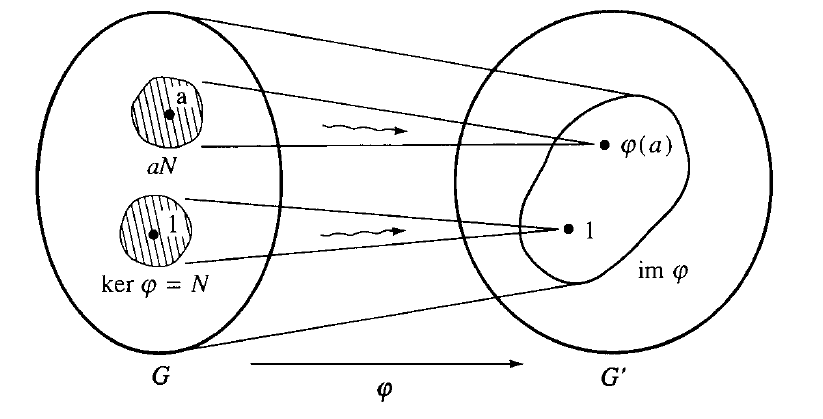
\includegraphics[width=\linewidth]{resources/img/group_homomorphism_schematic.png}
			\caption{A schematic diagram of a group homomorphism}
		\end{figure}
	
		\subsubsection{Congruence}
		Since a homomorphism maps the identity to the identity and inverses to inverses (\autoref{prop:isomorphism_preserves_structure}), we can deduce that the inverse image of the identity in $G'$ is going to contain at least the identity of $G$ and that the inverse image of an element $\inv{(a')} \in G'$ will contain at least the element $\inv{a} \in G$. So, in terms of equivalence classes we can say that, for a homomorphism $\phi$,
		\[ 1 = e \in \inv{\phi}(1') \implies \overline{\phi}(\overline{1}) = 1' \]
		\[ \inv{a} \in \inv{\phi}(\inv{(a')}) \implies \overline{\phi}(\overline{\inv{a}}) = \inv{(a')} \]

		\boxeddefinition{The equivalence relation determined by a homomorphism is known as \textbf{congruence} and is commonly denoted using $\equiv$ instead of $\sim$. For a homomorphism $\phi$,
			\[ a \equiv b \iff \phi(a) = \phi(b). \]
			Since $\phi$ is a homomorphism we also have,
			\[ a \equiv b \iff \phi(ac) = \phi(bc), \; \phi(\inv{a}) = \phi(\inv{b}). \]
			More generally, a \textbf{congruence relation} is an equivalence relation on an algebraic structure (such as a group, ring, or vector space) that is compatible with the structure in the sense that algebraic operations done with equivalent elements will yield equivalent elements.
		}
		\subsubsection{Congruence Examples}
		\begin{exe}
			\ex{The modulus function of complex numbers forms a homomorphism from the multiplicative group of complex numbers to the multiplicative group of reals,
				\[ \phi : \C{\times} \longmapsto \R{\times} \suchthat \phi(a) = \abs{a} \]
				and the induced equivalence relation is $a \equiv b \iff \abs{a} = \abs{b}$. The fibres of this map are the concentric circles about 0. They are in bijective correspondence with elements of $im \; \phi$, the set of positive reals.
			}
		\end{exe}
	
		\labeledProposition{If $\phi : G \longmapsto G'$ is a group homomorphism with kernel $N$ then, for $a,b \in G$,
			\[\phi(a) = \phi(b) \iff \exists n \in N, \suchthat b = an  \]
			or, equivalently, $\inv{a}b \in N$.
		}{kernel_elements_relate_congruent_elements}
		\begin{proof}
			\begin{align*}
				&& b &= an  \\
				&\implies & \phi(b) &= \phi(an) \\
				&\implies & \phi(b) &= \phi(a)\phi(n) &\sidecomment{by homomorphism property} \\
				&\implies & \phi(b) &= \phi(a)1' &\sidecomment{n is in the kernel} \\
				&\implies & \phi(b) &= \phi(a) \\
			\end{align*}
			\begin{align*}
				&& \phi(b) &= \phi(a) \\
				&\implies & \inv{\phi(a)}\phi(b) &= 1'  &\sidecomment{codomain is a group so has inverses} \\
				&\implies & \phi(\inv{a})\phi(b) &= 1' &\sidecomment{by \autoref{prop:isomorphism_preserves_structure}} \\
				&\implies & \phi(\inv{a}b) &= 1' &\sidecomment{by homomorphism property} \\
				&\implies & \inv{a}b &= n \in N \\
				&\implies & b &= an \\
			\end{align*}
		\end{proof}
	
		\begin{corollary}
			A group homomorphism is injective if and only if its kernel is the trivial subgroup $\{1\}$. So, a homomorphism is an isomorhpism if its kernel contains only the identity and its image is the whole of the codomain (i.e. it's surjective). 
		\end{corollary}
	}

	
	\pagebreak
	\searchableSubsection{Cosets}{abstract algebra}{\bigskip
		The set of elements of the form $an$ - described in \autoref{prop:kernel_elements_relate_congruent_elements} - is denoted by $aN$ and is called a \textit{coset} of $N$ in $G$.\\\\
		\boxeddefinition{A coset can be defined for any subgroup $H$ of a group $G$. A \textbf{left coset} is a subset of the form,
			\[ aH = \setc{ah}{h \in H}. \]
		}
		\note{Cosets are not, in general, subgroups. This can be easily seen as the left coset $aH$ does not contain the identity as, although $H$ contains the identity, $aH$ contains ${ a1 = a }$.} 
		Note that the arbitrary subgroup $H$ could also be thought of as a coset $1H = H$ and also that the left cosets $aH$ are equivalence classes for the congruence relation,
			\[ a \equiv b \iff b = ah, \; h \in H. \]
		This is a congruence because, for some arbitrary $c \in G$,
			\[ 1 \equiv c \iff \exists h \in H \suchthat c = 1h = h. \]
		That's to say, the elements that are congruent to the identity are precisely the members of the subgroup $H$ so that it plays a similar role to the kernel $N$ in \autoref{prop:kernel_elements_relate_congruent_elements}. Furthermore, since the congruence relation is an equivalence relation it forms a partition of the domain $G$.
		
		\labeledProposition{The left cosets of a subgroup partition the group.}{cosets_partition_group}
		\begin{proof}
			The left cosets are equivalence classes and, as a result, they partition the group.
		\end{proof}
	
		\subsubsection{Examples of cosets}
		\begin{exe}
			\ex{The coset of an element with the kernel $N$,
				\[ aN = \setc{g \in G}{g = an, \; n \in N} \]
				is the set of all elements that are \textit{congruent} to $a$. The \textit{congruence classes} are precisely the cosets $aN$ for each $a \in G$. They are also the \textit{fibres} of the homomorphic map.
			}\label{ex_coset_with_kernel}
			\ex \ref{S_3} Continuing the example of the symmetric group $S_3$ represented as 
				\[ G = \{1, x, x^2, y, xy, x^2y\} \]
				with group multiplication rules, 
				\[ x^3 = 1, y^2 = 1, yx = x^2y. \]
				The element $xy$ has order 2 so it generates a cyclic subgroup $H = \{1, xy\}$ of order 2. The left cosets of $H$ in $G$ are the three sets,
				\[ \{1,xy\} = 1H = xyH, \; \{x, x^2y\} = xH = x^2yH, \; \{x^2, y\} = x^2H = yH. \]
				Note that they do partition the group $G$. Also, notice that the cosets $aH$ for $a \in H$ produce the subgroup $H$ itself as should be expected as the group properties of the subgroup dictate that all products of its elements are already present in the subgroup. For this reason, the cosets $aH$ that are distinct from $H$ are those such that $a \not\in H$.\label{ex_S_3}
		\end{exe}
	
		\subsubsection{The index of a subgroup}
		\boxeddefinition{The \textbf{index} of a subgroup is the number of left cosets it forms in the parent group.}
		\notation{The \textbf{index} of a subgroup $H$ in $G$ is denoted by $[G:H]$.}
		\\\\
		In the example (\ref{ex_S_3}) the index of $H$ is 3. Note that if $G$ were to contain infinitely many elements then the index of a subgroup may also be infinite.\\
		
		\labeledProposition{Each coset $aH$ has the same number of elements as $H$.}{coset_cardinality_equal_to_subgroup}
		\begin{proof}
			As usual, equal cardinality is demonstrated by showing the existence of a bijection. It is clear that there is a bijective map between the subgroup $H$ and any coset $aH$ because the map $H \longmapsto aH$ is,
			\begin{itemize}
				\item{injective because $ah = ah' \implies h = h'$ because by group properties $a$ has an inverse in $G$;}
				\item{surjective because every $c \in aH$ has the form $ah$ and is therefore mapped to by some $h \in H$.}
			\end{itemize}
		\end{proof}
	
		\subsubsection{Lagrange's Theorem}
		Since the left cosets of $H$ in $G$ form a partition of $G$ and their order is the same as that of $H$ we see that the order of $G$ is the order of $H$ multiplied by its index in $G$. This results in a formula known as the \textit{Counting Formula} as follows,
		\[ \cardinality{G} = \cardinality{H} \cdot [G:H]. \]
		If $G$ is of infinite order and $H$ is finite, then the index of $H$ in $G$ will be infinite.
		
		\begin{theorem}
			\textbf{Lagrange's Theorem: } Let $G$ be a finite group, and let $H$ be a subgroup of $G$. The order of $H$ divides the order of $G$.
		\end{theorem}
	
		\begin{corollary}
			Let $ G $ be a finite group, and let $ a $ be an element of $ G $. Then the order of $ a $ divides the order of $G$. That's to say, the order of the cyclic group generated by $a$, ${ \cardinality{\langle a \rangle} }$, divides ${ \cardinality{G}. }$
		\end{corollary}
	
		\begin{corollary}
			\label{coro:group_order_n_nth_power_of_elements_is_identity}
			If $ G $ is a group of order $ n $, then ${ g^n = e }$ for every element $ g $ of $ G $.
		\end{corollary}
		\begin{proof}
			This is clearly a consequence of the previous corollary. If we let the order of $g$ be $m$, then by the previous corollary, 
			\[ m \divides n \iff n = km \text{ for } k \in \N{} \iff g^n = g^{km} = (g^m)^k = e^k = e. \qedhere \]
		\end{proof}
	
		\begin{corollary}
			\label{coro:prime_order_groups_are_cyclic}
			Suppose that a group $G$ has $p$ elements and that $p$ is a prime integer. Let $a \in G$ be any element, not the identity. Then $G$ is the cyclic group $\{1, a, \dots , a^{p-1}\}$ generated by $a$.
		\end{corollary}
		\begin{proof}
			Since $a \neq 1$ by selection, it has order greater than 1. Since its order must divide the order of $G$, which is prime, its order is equal to the order of $G$, $p$. So, the order of the nonidentity element $a$ is the same as the order of $G$ and so it generates the whole group.
		\end{proof}
	
		\begin{corollary}
			All groups with some prime order, $p$, are in the same isomorphism class.
		\end{corollary}
		\begin{proof}
			Any group with prime order $p$ is the cyclic group of order $p$ and by \autoref{prop:one_class_per_cyclic_order} there is only a single isomorphism class for each cyclic group of a given order.
		\end{proof}
	
		\subsubsection{Example applications of Lagrange Theorem}
		\begin{exe}
			\ex{\textbf{Fermat's Little Theorem}: \textit{If $ p $ is a prime number then \[ a^p \equiv a \bmod p \text{ for all } a \in \Z{}. \]}
				\note{
					We need to be a little careful here. We might assume -- given that we are multiplying the integer $a$ in modulo $p$ that the group we want to use is ${ (\Z{}_p, \otimes) }$. However, \textit{this is not a group!} The reason is that $\Z{}_p$ contains 0 which has no inverse under the proposed law of composition, multiplication.\\
					If, however, we take ${ \Z{*}_p }$ where the $*$ means ${ \Z{}/\{0\} }$ then we have a set of ${ p - 1 }$ distinct elements. Over this set we can form the multiplicative group ${ G = (\Z{*}_p, \otimes) }$ because the primality of $p$ means that every element has a multiplicative inverse.\\
					Note that this is \textbf{not} a group of prime order. The primality of $p$ is essential to make sure that every element has a multiplicative inverse but, since we also have to eliminate 0 for the same reason, the order is ${ p - 1 }$ which is not necessarily prime.
				}
				\begin{proof}
					Take the set ${ \Z{*}_p }$ under multiplication and some arbitrary ${ a \in \Z{} }$.
					\begin{enumerate}[label=(\roman*)]
						\item{Primality of $ p $ means that it is possible to find ${ 1 = na + mp }$ for ${ m,n \in \Z{} }$ (see \autoref{coro:greatest_common_divisor}). This implies that there exists a multiplicative inverse of every non-zero element in modulo $ p $. Specifically, $ n $ is the inverse of $ a $ because ${ na = (-m)p + 1 \iff na \bmod p \equiv 1}$.}
						\item{Existence of the multiplicative inverses implies that we have a group ${ G = (\Z{*}_p, \otimes) }$.}
						\item{$G$ being a group implies that, for any element ${ a \in G }$, by \autoref{coro:group_order_n_nth_power_of_elements_is_identity} we have ${ a^{p-1} = 1 }$.}
						\item{In $G$, ${ a^{p-1} = 1 \iff a^p = a }$ which translates to ${ a^p \equiv a \bmod p }$.}
					\end{enumerate}
				\end{proof}
			}
		\end{exe}
		
		\subsubsection{Lagrange's Theorem and Homomorphisms}
		The Counting Formula can also be applied when a homomorphism is given. Let $\phi : G \longmapsto G'$ be a homomorphism. As we saw in coset example \ref{ex_coset_with_kernel}, the left cosets of $ker \; \phi$ are the fibres of the map $\phi$. They are in bijective correspondence with the elements of the image. Therefore,
		\[ [G : ker \; \phi] = \cardinality{im \; \phi}. \]
		Which implies that,
		\begin{corollary}
			If $\phi : G \longmapsto G'$ is a homomorphism of finite groups then,
			\[ \cardinality{G} = \cardinality{ker \; \phi} \cdot \cardinality{im \; \phi}. \]
			As a result, $\cardinality{ker \; \phi}$ divides $\cardinality{G}$, and $\cardinality{im \; \phi}$ divides both $\cardinality{G}$ and $\cardinality{G'}$.
		\end{corollary}
	
		\subsubsection{Right Cosets}
		Right cosets also exist and are defined as,
		 \[ Ha = \setc{g \in G}{g = ha, \; h \in H} \]
		and these are equivalence classes for the \textit{right congruence} relation,
		\[ a \equiv b \iff b = ha, \; h \in H. \]
		Right cosets are not necessarily the same as left cosets. For instance, continuing the example in \ref{ex_S_3}, the right cosets of the subgroup $\{1, xy\}$ of $S_3$ are,
		\[ \{1, xy\} = H1 = Hxy, \; \{x, y\} = Hx = H, \; \{x^2, x^2y\} = Hx^2 = Hx^2y. \]
		Note that this generates a different partition of $G$ then was generated by the left cosets.
		
		\labeledProposition{A subset $H$ of a group $G$ is normal if and only if every left coset is also a right coset. If $H$ is normal then,
			 \[ \forall a \in G, \, aH = Ha. \]}{normal_subgroups_equal_cosets}
		\begin{proof}
			Suppose that $H$ is normal. For any $h \in H$ and any $a \in G$,
			\[ ah = (ah\inv{a})a. \]
			Since $H$ is normal, the conjugate by $h$ of $a$ is also in $H$, that's to say, $ ah\inv{a} \in H $ which implies that $ (ah\inv{a})a \in Ha $. Therefore, any arbitrary member of $aH$ is also a member of $Ha$. Clearly, the same proof also works in the other direction so that any member of $Ha$ is also a member of $aH$ and the two cosets are equal. So, we have shown that ($H$ is normal) $\implies$ (left and right cosets of $H$ are equal). \\
			Now we need to show that (left and right cosets of $H$ are equal) $\implies$ ($H$ is normal). Firstly, clearly the above logic doesn't apply if $H$ is not normal; there will be at least one element whose conjugate is not in $H$ so $aH \neq Ha$. However, it could still be the case that each left coset is also a right coset if, for every $a$ in $G$, there is some $b$ in $G$ such that $aH = Hb$. However, this is not possible because $aH$ and $Ha$ both contain $a$ which means that in a given partition of $G$ they must be the same partition. So $aH \neq Ha$ implies that the partitions are different; $Ha$ creates different equivalence classes. Therefore  (left and right cosets of $H$ are equal) $\implies$ ($H$ is normal).
		\end{proof} 
	}
	
	
	
	\pagebreak
	\searchableSubsection{\sectionTitle{Fields}}{abstract algebra}{\bigskip}
		
		\bigskip
		\searchableSubsection{Complex Numbers}{abstract algebra, complex numbers}{\bigskip
			\labeledProposition{For every $\alpha \in \C{}$, there exists a unique $\beta \in \C{}$ such that $\alpha + \beta = 0$.}{unique_complex_additive_inverse}
			\begin{proof}
			By contradiction: Say there are two such elements, $\beta, \gamma$ such that,
			\begin{align*}
			\alpha + \beta &= 0 = \alpha + \gamma \\
			(\alpha + \beta) + \beta &= (\alpha + \beta) + \gamma \\
			0 + \beta &= \beta = 0 + \gamma = \gamma \qedhere\\
			\end{align*}
			\end{proof}
			
			\labeledProposition{For every $\alpha \in \C{}$ with $\alpha \neq 0$, there exists a unique $\beta \in \C{}$ such that $\alpha\beta = 1$.}{unique_complex_multiplicative_inverse}
			\begin{proof}
			By contradiction: Say there are two such elements, $\beta, \gamma$ then,
			\begin{align*}
			\alpha\beta &= 1 = \alpha\gamma \\
			\beta &= \frac{1}{\alpha} = \gamma \qedhere\\
			\end{align*}
			\end{proof}
		}
		
		\bigskip\bigskip
		\searchableSubsection{Complex Numbers Problems}{abstract algebra, complex numbers}{\bigskip\bigskip}
		
		\searchable{subsubsection}{Find all the roots of $x^3 = 1$ for $x \in \C{}$}{complex numbers}{
		Since $x^3 - 1 = (x - 1)(x^2 + x + 1)$, we have (via zero-factor theorem) possible roots from,
		\[ x - 1 = 0 \iff x = 1 \]
		\begin{align*}
		x^2 + x + 1 &= 0
		\implies x = \frac{-1 \pm \sqrt{-3}}{2} = \frac{-1 \pm \sqrt{3}\,i}{2}
		\end{align*}
		More generally,
		\[ (a+bi)+(a-bi)=2a \] 
		and since also,
		\[ \left[\frac{-1 + \sqrt{3}\,i}{2}\right]^2 = \frac{-1 - \sqrt{3}\,i}{2} \]
		as well as the reverse,
		\[ \left[\frac{-1 - \sqrt{3}\,i}{2}\right]^2 = \frac{-1 + \sqrt{3}\,i}{2} \]
		this means that if $x = \frac{-1 \pm \sqrt{3}\,i}{2}$ then $x^2 + x$ is of the form $(a+bi)+(a-bi) = 2a$ and so we have that $x^2 + x = -1 \iff x^2 + x + 1 = 0$.\\\\
		In addition,
		\[ (a+bi)(a-bi)=a^2+b^2 \]
		which means that if $x = \frac{-1 \pm \sqrt{3}\,i}{2}$ then $x^3 = x^2x$ is of the form $(a+bi)(a-bi)=a^2+b^2$ so we have
		that $x^3 = {\frac{-1}{2}}^2 + {\frac{\sqrt{3}}{2}}^2 = \frac{1}{4} + \frac{3}{4} = 1$.\\\\
		So we see that - allowing for complex $x$ - the cubic polynomial $x^3 - 1$ has 3 roots as we should expect from the \href{https://en.wikipedia.org/wiki/Fundamental_theorem_of_algebra}{Fundamental Theorem of Algebra} \textit{\color{red}{(is this the correct interpretation of this?)}}.
		}

\end{document}